% Harus dimuat terlebih dahulu, digunakan agar file PDF memiliki format karakter yang benar.
% Untuk informasi lebih lanjut, lihat https://ctan.org/pkg/cmap.
\RequirePackage{cmap}

% Format dokumen sebagai paper konferensi menggunakan aturan IEEEtran terbaru (v1.8b).
% Untuk informasi lebih lanjut, lihat http://www.michaelshell.org/tex/ieeetran/.
\documentclass[conference]{IEEEtran}[2015/08/26]

% Format encoding font dan input menjadi 8-bit UTF-8.
\usepackage[T1]{fontenc}
\usepackage[utf8]{inputenc}

% Format bahasa menjadi bahasa german dan inggris.
\usepackage[english]{babel}

% Digunakan untuk tujuan demonstrasi.
\usepackage{mwe}

% Digunakan untuk menampilkan font dengan style yang lebih baik.
\usepackage[zerostyle=b,scaled=.75]{newtxtt}

% Digunakan untuk menampilkan tabel dengan style yang lebih baik.
\usepackage{booktabs}
\usepackage[table,xcdraw]{xcolor}
% Digunakan untuk menampilkan gambar pada dokumen.
\usepackage{graphicx}

\usepackage{longtable}
\usepackage{tabularx}
\usepackage{multicol}
\usepackage{float}
\usepackage{multirow}
% \usepackage[table,xcdraw]{xcolor}

% Digunakan untuk menampilkan potongan kode.
\usepackage{listings}
\lstset{
  basicstyle=\ttfamily,
  columns=fixed,
  basewidth=.5em,
  xleftmargin=0.5cm,
  captionpos=b
}

% Digunakan agar backticks (`) dapat dirender pada PDF.
% Untuk informasi lebih lanjut, lihat https://tex.stackexchange.com/a/341057/9075.
\usepackage{upquote}

% Digunakan untuk menyeimbangkan bagian akhir dokumen dengan dua kolom.
\usepackage{balance}

% Digunakan untuk menampilkan pustaka.
\usepackage[square,comma,numbers,sort&compress]{natbib}

% Mengubah format ukuran teks pada natbib.
\renewcommand{\bibfont}{\normalfont\footnotesize}

% Menambah nama penulis ketika menggunakan perintah \citet.
% Untuk informasi lebih lanjut, lihat https://tex.stackexchange.com/a/76075/9075.
\usepackage{etoolbox}
%\makeatletter
%\patchcmd{\NAT@test}{\else \NAT@nm}{\else \NAT@hyper@{\NAT@nm}}{}{}
%\makeatother

% Digunakan untuk melakukan linewrap pada pustaka dengan url yang panjang
% jika terdapat hyphens
\usepackage[hyphens]{url}

% Digunakan untuk menambah hyperlink pada referensi.
\usepackage{hyperref}

% Menonaktifkan warna dan bookmark pada hyperref.
\hypersetup{hidelinks,
  colorlinks=true,
  allcolors=black,
  pdfstartview=Fit,
  breaklinks=true
}

% Digunakan untuk membenarkan hyperref pada gambar.
\usepackage[all]{hypcap}

% Digunakan untuk menampilkan beberapa gambar
\usepackage[caption=false,font=footnotesize]{subfig}

\usepackage{stfloats}

% Tambahkan format tanda hubung yang benar di sini
\hyphenation{
  ro-ket
  me-ngem-bang-kan
  per-hi-tu-ngan
}

\begin{document}

  % Ubah kalimat berikut sesuai dengan judul penelitian.
\title{Kalkulasi Energi pada Roket Luar Angkasa \\ Berbasis \emph{Anti-Gravitasi}}

% Ubah kalimat-kalimat berikut sesuai dengan nama, institusi, alamat dan kontak penulis.
\author{
  \IEEEauthorblockN{Elon Reeve Musk}
  \IEEEauthorblockA{Departemen Teknik Dirgantara\\
    Fakultas Teknologi Dirgantara\\
    Institut Teknologi Sepuluh Nopember\\
    Surabaya, Indonesia 60111\\
    elon.musk@mhs.its.ac.id}

  \and
  \IEEEauthorblockN{Nikola Tesla}
  \IEEEauthorblockA{Departemen Teknik Dirgantara\\
    Fakultas Teknologi Dirgantara\\
    Institut Teknologi Sepuluh Nopember\\
    Surabaya, Indonesia 60111\\
    \url{https://nikolatesla.me}}

  \and
  \IEEEauthorblockN{Wernher von Braun}
  \IEEEauthorblockA{Departemen Teknik Dirgantara\\
    Fakultas Teknologi Dirgantara\\
    Institut Teknologi Sepuluh Nopember\\
    Surabaya, Indonesia 60111\\
    von.braun@td.its.ac.id}
}

% Digunakan untuk menampilkan judul dan deskripsi penulis.
\maketitle

  % Mengubah keterangan `Abstract` ke bahasa indonesia.
% Hapus bagian ini untuk mengembalikan ke format awal.
\renewcommand\abstractname{Abstrak}

\begin{abstract}

  Diabetic retinopathy (DR) is a microvascular complication of diabetes and is the leading cause of blindness among working-age adults worldwide. Early detection and intervention are crucial to prevent vision loss and improve patient outcomes. However, traditional screening methods often face limitations in accuracy and accessibility. This study proposes the implemen-tation of a Residual Neural Network (ResNet) for automated DR detection and classification from fundus images. By achieving these objectives, this study aims to contribute to the advance-ment of automated DR diagnosis and ultimately improve patient care through early intervention and personalized treatment strategies.The most accurate model, ResNet-18, achieved the best validation accuracy without any adjustment to the class weight, with a value of 0.8211. Addi-tionally, the model with the highest Kappa score was ResNet-18, which had the best training accuracy without any modification to the class weight, resulting in a Kappa score of 0.7584.

\end{abstract}

% Mengubah keterangan `Index terms` ke bahasa indonesia.
% Hapus bagian ini untuk mengembalikan ke format awal.
\renewcommand\IEEEkeywordsname{Keywords}

\begin{IEEEkeywords}

  % Ubah kata-kata berikut sesuai dengan kata kunci dari penelitian.
  Diabetic retinopathy, ResNet, Deep Learning, Optical Coherence Tomography Angiography Analysis.

\end{IEEEkeywords}


  % Ubah bagian berikut sesuai dengan konten-konten yang akan dimasukkan pada dokumen
  % Ubah judul dan label berikut sesuai dengan yang diinginkan.
\section{Introduction}
\label{sec:pendahuluan}

% Ubah paragraf-paragraf pada bagian ini sesuai dengan yang diinginkan.

In the present age of digital technology, artificial intelligence has become intimately intertwined with several facets of human life. These advancements in technology have had a positive impact on various aspects of our lives. They have enhanced productivity by providing content recommendations on social media, virtual assistants, and spam filters. Additionally, they have improved efficiency through the implementation of intelligent transportation systems and automatic scheduling. Furthermore, they have contributed to entertainment and have played a significant role in the research and development sector of science and technology.
 
Diabetic retinopathy is a consequence of diabetes mellitus (DM) that occurs when blood vessels in the retina are damaged. The condition can result in diminished eyesight and potentially complete loss of vision \citet{Yusran2022}.

Approximately 9.3 million individuals worldwide are afflicted with blindness caused by diabetic retinopathy, as reported by the World Health Organization (WHO). The projected figure is anticipated to rise to 12.6 million by the year 2040.

Early detection of diabetic retinopathy is essential in order to avoid the advancement of the illness and minimize the likelihood of severe consequences. Technology, particularly in the field of medical image processing, is now essential in the medical industry to enhance the early diagnosis of diabetic retinopathy. The Residual Neural Network (ResNet) is a well-established approach with numerous tools available for in-depth study.

ResNet is a neural network specifically created to tackle the issue of declining performance in neural networks with more depth. The residual technique enables ResNet to effectively optimize network learning on intricate data, such as medical images. The objective of this study is to examine diabetic retinopathy using a Convolutional Artificial Neural Network. 


This paper commences with a presentation of other research (Section \ref{sec:relatedresearch}).
This is followed by an explanation of the system architecture (Section \ref{sec:architecture}).
Based on the aforementioned findings, we present the results obtained in (Section \ref{sec:results}).
Finally, we present our conclusions based on the research conducted (Section \ref{sec:conclusion}).
  % Ubah judul dan label berikut sesuai dengan yang diinginkan.
\section{Penelitian Terkait}
\label{sec:penelitianterkait}

\subsection{\emph{Classification of Diabetic Retinopathy Based on B-ResNet}}
\label{subsec:penelitianTerdahulu1}
Zhang dan rekan \citet{zhang2022residual} pada penelitiannya menggunakan data set Eye-PACS, MESSIDOR-2, dan IDRiD untuk membangun data set DR dengan pembersihan, penguatan, dan normalisasi gambar. Selain itu, digunakan metode prapemrosesan gambar yang ditingkatkan untuk meningkatkan fitur gambar fundus. Model B-ResNet dibangun dengan menggabungkan keunggulan ekstraksi fitur ResNet50 dan fusi fitur BCNN. Selain itu, sebelum fusi fitur, gambar fitur yang diekstraksi oleh ResNet50 diproses oleh modul perhatian saluran. ResNet50 dipralatih pada data set ImageNet dan parameternya di-fine-tune melalui transfer learning.

Hasil penelitian menunjukkan bahwa model B-ResNet mencapai akurasi 71,11\% , ACA 0,714, Kappa 0,634, dan macro-F1 0,711. Hasil ini lebih tinggi daripada penelitian sebelumnya. Percobaan perbandingan membuktikan bahwa metode prapemrosesan gambar yang ditingkatkan meningkatkan akurasi, ACA, Kappa, dan nilai macro-F1 model.

\subsection{\emph{A Deep Learning Framework for Detection and Classification of Diabetic Retinopathy in FundusImages Using Residual Neural Networks}}
\label{subsec:penelitianTerdahulu2}
Abini dan rekan \citet{10335079} melakukan studi menggunakan model ResNet, yang dilatih dengan dataset APTOS, untuk melakukan klasifikasi biner dan multikelas menggunakan jaringan saraf konvolusional dalam (deep convolutional neural network). Hasil eksperimen menunjukkan bahwa model dengan lapisan dalam seperti ResNet-50 dapat meningkatkan kinerja keseluruhan dataset. Ini mengindikasikan bahwa penggunaan model ResNet-50 dalam klasifikasi DR dapat menjadi lebih efisien dalam hal waktu, tenaga kerja, dan biaya dibandingkan dengan metode diagnostik manual.

  % Ubah judul dan label berikut sesuai dengan yang diinginkan.
\section{Arsitektur}
\label{sec:arsitektur}

% Ubah paragraf-paragraf pada bagian ini sesuai dengan yang diinginkan.

\subsection{Dataset Penelitian}
\label{subsec:dataset}

Data yang digunakan dalam penelitian ini adalah data yang diperoleh dari Diabetic Retinopathy Analisis Grand challenge, berupa citra OCT-\emph{Angiography}.
Untuk persebaran data yang digunakan pada penelitian ini, terdapat pada tabel \ref{table:Datasettraining}

	\begin{figure}[hbtp]
		\centering
		\subfloat[\centering Non-DR]{{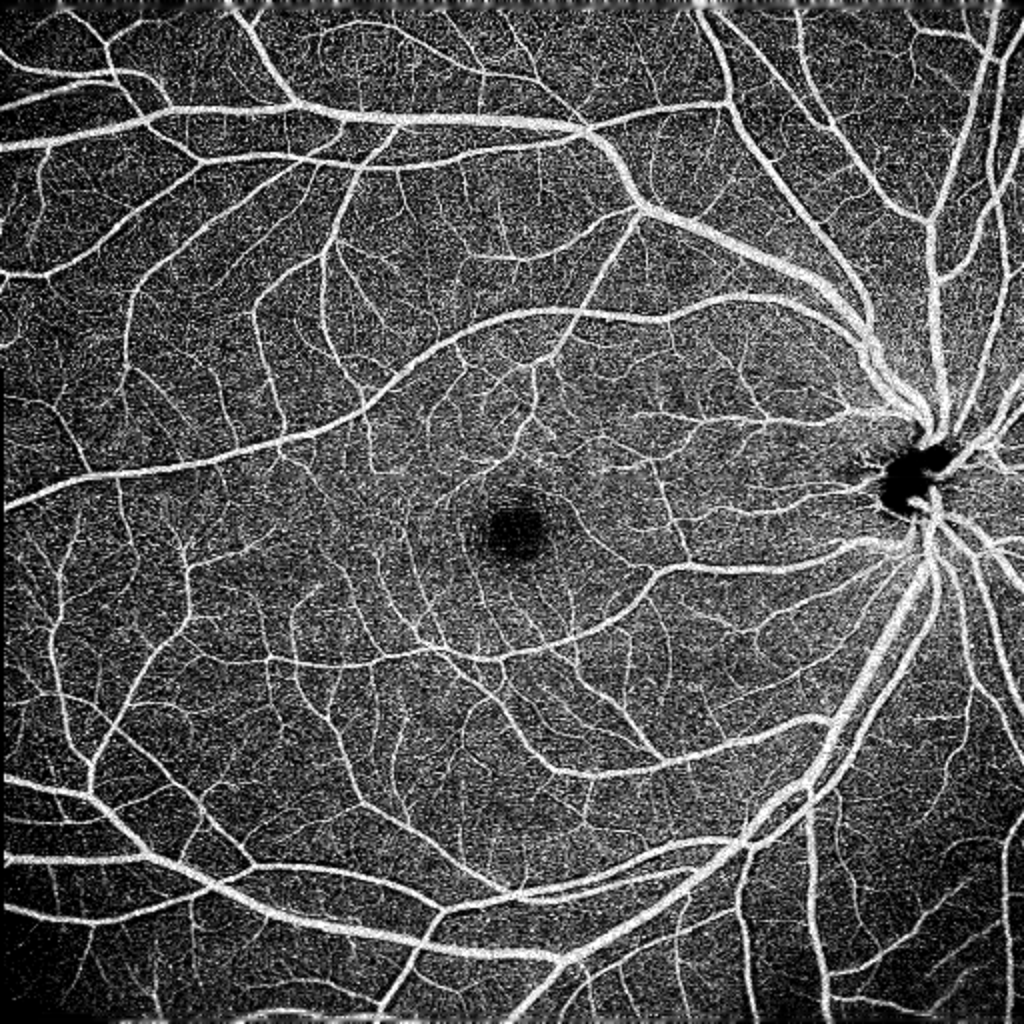
\includegraphics[width=2.5cm]{gambar/non-DR.png} }}%
		\subfloat[\centering NPDR]{{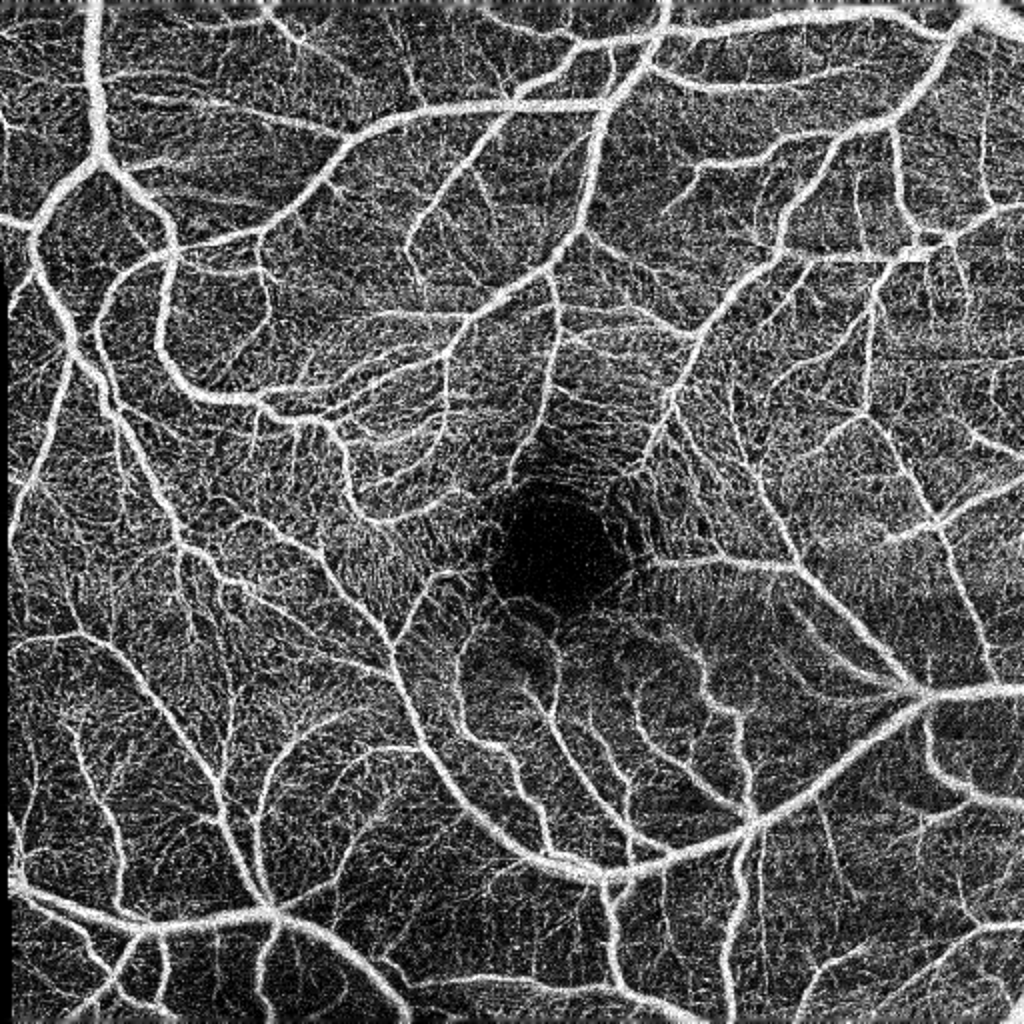
\includegraphics[width=2.5cm]{gambar/NPDR.png} }}%
		\subfloat[\centering PDR]{{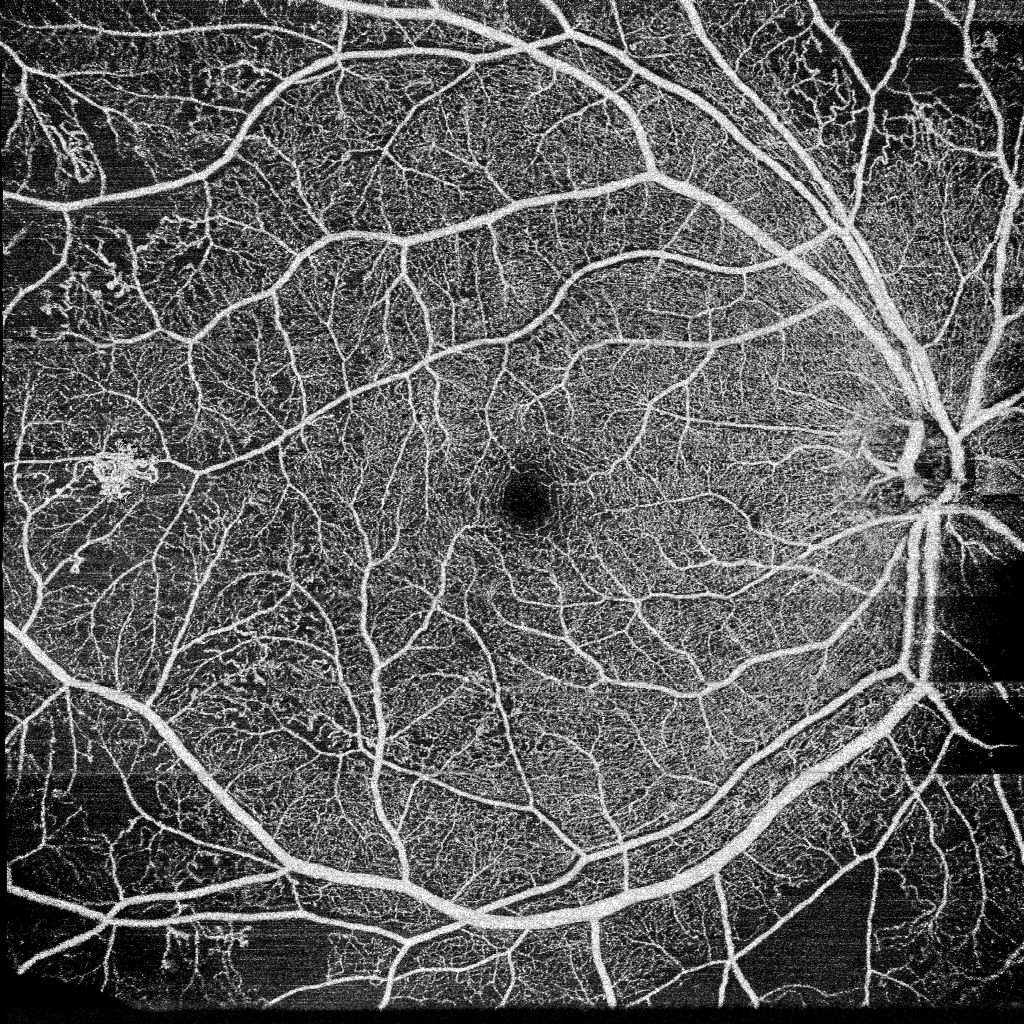
\includegraphics[width=2.5cm]{gambar/PDR.png} }}%
		\caption{Contoh Data Citra Retina}
		\label{fig:sampleDataset}
	\end{figure}
Gambar yang diberikan adalah foto fundus retina yang digunakan untuk evaluasi retinopati diabetik. Foto ini menunjukkan detail dari jaringan pembuluh darah retina, disk optik, dan area makula. Berikut adalah deskripsi rinci dari gambar tersebut:

Informasi Dataset dari Tantangan DRAC
Dataset yang digunakan untuk pelatihan dan pengujian terdiri dari:

	\begin{itemize}
		\item Set Pelatihan: 611 gambar
		\item Set Uji: 386 gambar
	\end{itemize}
Gambar-gambar pada set pelatihan, kemudian dipisah kembali menjadi dua set, yaitu set untuk pelatihan dan set untuk validasi dengan jumlah sesuai pada tabel \ref{table:Datasettraining}

%\begin{table}[hbtp]
%	\begin{center}
%	\caption{Tabel distribusi Set untuk Pelatihan dan Validasi}
%	\label{table:Datasettraining}
%	\begin{tabular}{|l|l|l|l|}
%		\hline
%		\rowcolor[HTML]{C0C0C0} 
%		Label                                                & Klasifikasi & Jumlah & Total                                         \\ \hline
%		\rowcolor[HTML]{FFFFFF} 
%		\cellcolor[HTML]{FFFFFF}                             & non-DR      & 263    & \cellcolor[HTML]{FFFFFF}                      \\ \cline{2-3}
%		\rowcolor[HTML]{FFFFFF} 
%		\cellcolor[HTML]{FFFFFF}                             & NPDR        & 169    & \cellcolor[HTML]{FFFFFF}                      \\ \cline{2-3}
%		\rowcolor[HTML]{FFFFFF} 
%		\multirow{-3}{*}{\cellcolor[HTML]{FFFFFF}Training}   & PDR         & 56     & \multirow{-3}{*}{\cellcolor[HTML]{FFFFFF}488} \\ \hline
%		\rowcolor[HTML]{FFFFFF} 
%		\cellcolor[HTML]{FFFFFF}                             & non-DR      & 66     & \cellcolor[HTML]{FFFFFF}                      \\ \cline{2-3}
%		\rowcolor[HTML]{FFFFFF} 
%		\cellcolor[HTML]{FFFFFF}                             & NPDR        & 43     & \cellcolor[HTML]{FFFFFF}                      \\ \cline{2-3}
%		\rowcolor[HTML]{FFFFFF} 
%		\multirow{-3}{*}{\cellcolor[HTML]{FFFFFF}Validation} & PDR         & 14     & \multirow{-3}{*}{\cellcolor[HTML]{FFFFFF}123} \\ \hline
%		\end{tabular}
%	\end{center}
%\end{table}

Sedangkan gambar pada set uji digunakan untuk mendapatkan penilaian online menggunakan metrik Quadratic Weighted Kappa dengan model dari DRAC sebagai pembandingnya. dan dikarenakan set uji yang diberikan ini tidak memiliki label, maka set ini tidak dapat dipergunakan untuk pengambilan metrik lain seperti \emph{precision, recall}, dan \emph{F1-score}.

\subsection{Methodology}
\label{subsec:loremipsum}

Perbandingan metode skenario yang digunakan dalam pelatihan model ResNet:
Dalam penelitian ini, dikarenakan oleh dataset yang sedikit dan ada class yang kurang representatif, dilakukan beberapa metode untuk penyeimbangan dataset.
\begin{itemize}
	\item Default
	
	Tidak ada Tindakan yang dilakukan untuk menyeimbangkan dataset. Metode ini dilakukan untuk variabel kontrol
	\item Penyesuaian \emph{Class-weight}
	
	Pada metode ini, dilakukan penambahan weight agar class yang underrepresented memiliki beban lebih tinggi
\end{itemize}

\begin{figure}[hbtp] \centering
	% Nama dari file gambar yang diinputkan
	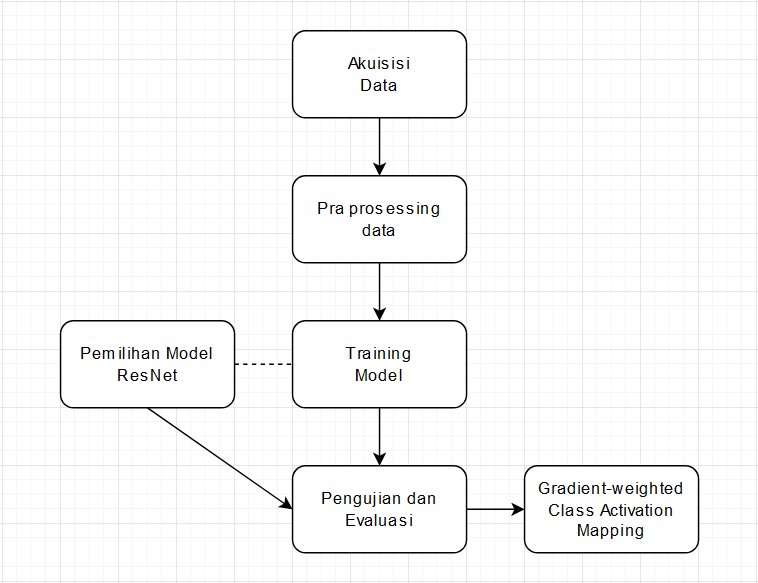
\includegraphics[scale=0.5]{gambar/diagramMethod.png}
	% Keterangan gambar yang diinputkan
	\caption{Diagram blok metodologi}
	% Label referensi dari gambar yang diinputkan
	\label{fig:diagramMethod}
\end{figure}

\subsection{Pelatihan Model}
\label{sec:325}
Pelatihan model dilakukan dengan menggunakan metode \emph{transfer learning}. Metode \emph{transfer learning} dilakukan dengan menggunakan model ResNet yang sudah dipilih dan sudah dilatih dengan dataset ImageNet.
Arsitektur model yang digunakan sesuai pada penjelasan bagian \ref{sec:323} dengan menggunakan \emph{hyper-parameter} yang ada pada tabel \ref{tb:hyperParameterTraining}
\begin{table}[hbtp]
	\begin{center}
		\caption{Hyperparameter}
		\label{tb:hyperParameterTraining}
		\begin{tabular}{|
		>{\columncolor[HTML]{C0C0C0}}l |l|lll}
		\cline{1-2}
		Input shape                                         & 224,224,3      &  &  &  \\ \cline{1-2}
		Opimizer                                            & Adam           &  &  &  \\ \cline{1-2}
		Loss Function                                       & Cross Entropy  &  &  &  \\ \cline{1-2}
		Learning Rate                                       & 0.1            &  &  &  \\ \cline{1-2}
		Momentum                                            & 0.9            &  &  &  \\ \cline{1-2}
		\cellcolor[HTML]{C0C0C0}                            & Step size = 10 &  &  &  \\ \cline{2-2}
		\multirow{-2}{*}{\cellcolor[HTML]{C0C0C0}Scheduler} & Gamma = 0.1    &  &  &  \\ \cline{1-2}
		Epoch                                               & 100            &  &  &  \\ \cline{1-2}
		Batch size                                          & 32             &  &  &  \\ \cline{1-2}
		\end{tabular}
	\end{center}
\end{table}


% Contoh pembuatan potongan kode.
%\begin{lstlisting}[
%  language=C++,
%  caption={Program halo dunia.},
%  label={lst:halodunia}
%]
%#include <iostream>
%
%int main() {
%    std::cout << "Halo Dunia!";
%    return 0;
%}
%\end{lstlisting}
  % Ubah judul dan label berikut sesuai dengan yang diinginkan.
\section{Result}
\label{sec:hasilPenelitian}



% Contoh input potongan kode dari file.
%\lstinputlisting[
%  language=Python,
%  caption={Program perhitungan bilangan prima.},
%  label={lst:bilanganprima}
%]{program/bilangan-prima.py}


  % Ubah judul dan label berikut sesuai dengan yang diinginkan.
\section{Kesimpulan}
\label{sec:kesimpulan}

Berdasarkan hasil penelitian yang telah dilakukan dapat ditarik kesimpulan-kesimpulan berikut:
Akurasi secara umum mengalami penurunan pada semua model, namun akurasi pada class PDR mengalami kenaikan terkecuali pada ResNet-50 yang tidak terdapat kenaikan maupun penurunan. Akurasi PDR pada ResNet-152 mengalami kenaikan yang paling signifikan, yaitu sebesar 0,428572. Pada metrik Quadratic Weighted Kappa, hanya resnet 18 dan 101 yang mengalami penurunan nilai.
Akurasi secara umum mengalami penurunan pada semua model, namun akurasi pada class PDR mengalami kenaikan terkecuali pada ResNet-18 yang tidak terdapat kenaikan maupun penurunan. Akurasi PDR pada ResNet-152 kembali mengalami kenaikan yang paling signifikan, yaitu sebesar 0,357143. Pada metrik QWK, hanya resnet 50 dan 101 yang mengalami kenaikan nilai.
Akurasi model secara umum mengalami penurunan kecuali pada model ResNet-18 dan ResNet-50. Sedangkan sama seperti model pada tabel-tabel sebelumnya, akurasi pada class PDR mengalami kenaikan dengan ResNet-50 mengalami kenaikan yang paling signifikan, yaitu sebesar 0,285715. Pada metrik QWK, hanya ResNet-101 dan ResNet-152 yang mengalami kenaikan nilai.


  % Menampilkan daftar pustaka dengan format IEEE
  \bibliographystyle{IEEEtranN}
  \bibliography{pustaka/pustaka.bib}

  % Menyeimbangkan bagian akhir di kedua kolom
  \balance

\end{document}
